\begin{tikzpicture}[
    node distance=14mm and 10mm,
    stage/.style={
        draw,
        rounded corners=2pt,
        semithick,
        align=center,
        minimum height=11mm,
        text width=20mm,
        fill=gray!8
    },
    snippetstage/.style={
        draw,
        line width=0.35pt,
        draw=black!30,
        minimum width=37mm,
        minimum height=24mm,
        fill=white
    },
    smstage/.style={
        draw,
        line width=0.35pt,
        draw=black!30,
        minimum width=37mm,
        minimum height=24mm,
        fill=white
    },
    vmstage/.style={
        draw,
        rounded corners=2pt,
        semithick,
        align=center,
        minimum height=30mm,
        text width=56mm,
        fill=gray!8
    },
    innerbox/.style={
        draw,
        align=center,
        fill=white,
        inner sep=3pt,
        text width=46mm
    },
    cell/.style={
        draw,
        minimum height=6mm,
        minimum width=12mm,
        align=center,
        fill=white,
        font=\ttfamily\scriptsize
    },
    tool/.style={
        draw,
        rounded corners=2pt,
        align=center,
        minimum height=8mm,
        text width=36mm,
        fill=white
    },
    flow/.style={->, semithick},
    attach/.style={->, dashed, semithick}
]

\node[snippetstage] (lama) {};
\node[stage, right=of lama, text width = 30mm] (compiler) {Компилятор\\байткода};
\node[smstage, right=of compiler] (bc) {};
\node[vmstage, right=of bc] (vm) {Виртуальная машина};
\node[anchor=north west, inner sep=0pt] at ($(lama.north west)+(0.8mm,-0.8mm)$) {
    \begin{tikzpicture}[x=1mm,y=-1mm]
        \clip (0,0) rectangle (36.4,21.9);
        \node[
            anchor=north west,
            align=left,
            font=\ttfamily\fontsize{4.6}{5.1}\selectfont
        ] at (0.05,0.05)
            {var x, y, z;\\
             \\
             fun zip (x) \{\\
             \ \ case x of Pair (x, y) ->\\
             \ \ \ \ case x of\\
             \ \ \ \ \ \ Nil          ->  Nil\\
             \ \ \ \ | Cons (x, xs) -> case y of\\
             \ \ \ \ \ \ \ \ \ \ \ \ \ \ \ Nil ->  Nil\\
             \ \ \ \ \ \ \ \ \ \ \ \ \ \ | Cons (y, ys) ->\\
             \ \ \ \ \ \ \ \ \ \ \ \ \ \ \ \ Cons (Pair (x, y),\\
             \ \ \ \ \ \ \ \ \ \ \ \ \ \ \ \ \ \ zip (Pair (xs, ys)))\\
             \ \ \ \ \ \ \ \ \ \ \ \ \ \ esac\\
             \ \ \ \ esac};
        \node[anchor=south east, font=\ttfamily\tiny, text=gray!65]
            at (36.8,21.5) {$\ddots$};
    \end{tikzpicture}
};
\node[anchor=north west, inner sep=0pt] at ($(bc.north west)+(0.8mm,-0.8mm)$) {
    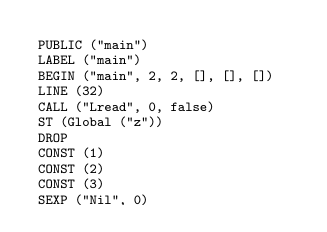
\begin{tikzpicture}[x=1mm,y=-1mm]
        \clip (0,0) rectangle (34.4,22.4);
        \node[
            anchor=north west,
            align=left,
            font=\ttfamily\fontsize{5.0}{5.6}\selectfont
        ] at (0.1,0.25)
            {PUBLIC ("main")\\
             LABEL ("main")\\
             BEGIN ("main", 2, 2, [], [], [])\\
             LINE (32)\\
             CALL ("Lread", 0, false)\\
             ST (Global ("z"))\\
             DROP\\
             CONST (1)\\
             CONST (2)\\
             CONST (3)\\
             SEXP ("Nil", 0)\\
             SEXP ("Cons", 2)};
    \end{tikzpicture}
};
\node[] at ([yshift=-11mm]vm.center) 
(ops)
{
    \begin{tikzpicture}[node distance=0mm]
        \node[cell] (c1) {insn$_1$};
        \node[cell, right=0mm of c1] (c2) {insn$_2$};
        \node[cell, right=0mm of c2, minimum width=8mm] (c3) {$\cdots$};
        \node[cell, right=0mm of c3] (c4) {insn$_n$};
    \end{tikzpicture}
};

\draw[flow] (lama) -- (compiler);
\draw[flow] (compiler) -- (bc);
\draw[flow] (bc) -- (vm);

\node[tool, below=16mm of lama, fill=green!12] (tool-lama) {\textsc{AFL++} \\Grammarinator};
\node[tool, below=16mm of bc, fill=orange!14] (tool-bc) {\textsc{AFL++}};
\node[tool, below=16mm of vm, fill=blue!10] (tool-cbmc) {\textsc{CBMC}};

\draw[attach] (tool-lama) -- (lama);
\draw[attach] (tool-bc) -- (bc);
\draw[attach] (tool-cbmc) -- (ops);

\node[font=\small, align=center, below=1mm of tool-lama] {фаззинг\\грамматики};
\node[font=\small, align=center, below=1mm of tool-bc] { фаззинг\\байткода};
\node[font=\small, align=center, below=1mm of tool-cbmc] {проверка инвариантов };

\end{tikzpicture}
